
\tikzstyle{startstop} = [rectangle, rounded corners, text centered, draw=black, fill=red!30]
\tikzstyle{process} = [rectangle, text centered, draw=black, fill=orange!30]
\tikzstyle{decision} = [rectangle, text centered, draw=black, fill=green!30]
\tikzstyle{arrow} = [thick,->,>=stealth]

\framebox{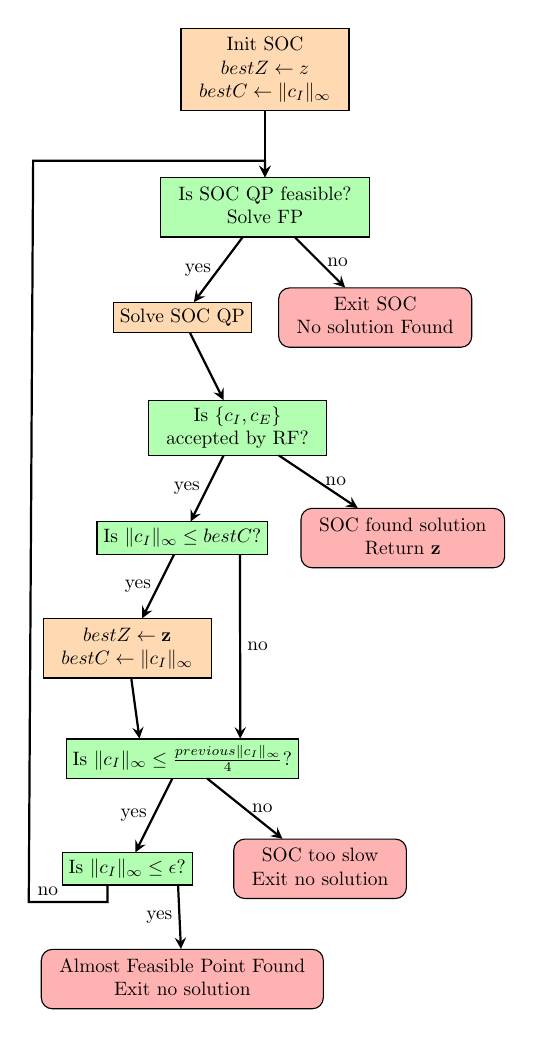
\begin{tikzpicture}[node distance=2cm, scale=0.7, every node/.style={transform shape}]

\node (init) [process] {\begin{tabular}{c}Init SOC\\ $bestZ\leftarrow z$\\ $bestC\leftarrow\|c_I\|_\infty$\end{tabular}};
\node (FPTest) [decision, below of=init, yshift=-5mm] {\begin{tabular}{c}Is SOC QP feasible?\\Solve FP\end{tabular}};
\node (noSolution) [startstop, below of=FPTest, xshift=2cm] {\begin{tabular}{c}Exit SOC\\No solution Found\end{tabular}};
\node (QP) [process, below of=FPTest, xshift=-15mm] {Solve SOC QP};
\node (filterTest) [decision, below of=QP, text width=3cm, xshift=10mm] {Is $\{c_I,c_E\}$ accepted by RF?};
\node (success) [startstop, below of=filterTest, xshift=30mm] {\begin{tabular}{c}SOC found solution\\Return $\bf z$\end{tabular}};
\node (betterViolTest) [decision, below of=filterTest, xshift=-10mm] {Is $\|c_I\|_\infty\leq bestC$?};
\node (updateBest) [process, below of=betterViolTest, xshift=-10mm] {\begin{tabular}{c}$bestZ\leftarrow \bf z$  \\ $bestC\leftarrow\|c_I\|_\infty$ \end{tabular}};
\node (tooSlowTest) [decision, below of=updateBest, xshift=10mm] {Is $\|c_I\|_\infty\leq \frac{previous \|c_I\|_\infty}{4}$?};
\node (almostFeasibleTest) [decision, below of=tooSlowTest, xshift=-10mm] {Is $\|c_I\|_\infty\leq\epsilon$?};
\node (tooSlowFail) [startstop, below of=tooSlowTest, xshift=25mm] {\begin{tabular}{c}SOC too slow\\Exit no solution\end{tabular}};
\node (almostFeasible) [startstop, below of=almostFeasibleTest, xshift=10mm] { \begin{tabular}{c}Almost Feasible Point Found\\Exit no solution\end{tabular} };

\draw [arrow] (init) -- (FPTest);
\draw [arrow] (FPTest) -- node[anchor=west] {no}  (noSolution);
\draw [arrow] (FPTest) -- node[anchor=east] {yes} (QP);
\draw [arrow] (QP) -- (filterTest);
\draw [arrow] (filterTest) -- node[anchor=west] {no} (success);
\draw [arrow] (filterTest) -- node[anchor=east] {yes}(betterViolTest);
\draw [arrow] (betterViolTest) -- node[anchor=east] {yes} (updateBest);
\draw [arrow] (betterViolTest.344) -- node[anchor=west] {no}(tooSlowTest.19);
\draw [arrow] (updateBest) -- (tooSlowTest.155);
\draw [arrow] (tooSlowTest) -- node[anchor=west] {no}(tooSlowFail);
\draw [arrow] (tooSlowTest) -- node[anchor=east] {yes}(almostFeasibleTest);
\draw [arrow] (almostFeasibleTest.342) --node[anchor=east] {yes} (almostFeasible);
\draw [arrow] (almostFeasibleTest.220) node[anchor=west, shift={(-14mm,-1mm)}] {no}|-([shift={(-6mm,-3mm)}]almostFeasibleTest.south west)-- ([shift={(-23mm,3mm)}]FPTest.north west)-| (FPTest);

\end{tikzpicture}}
